\chapter{Grundlagen des Spiels Vier Gewinnt}
Im Kapitel Grundlagen wird auf die Regeln des Spiels, sowie auf den geschichtlichen Hintergrund als auch die mathematischen Eigenschaften des Spiels 4Gewinnt genauer eingegangen. 

\section{Spielregeln und Spielablauf}
%Die Regeln für dieses Strategiespiel sind kinderleicht, was auch ein Argument für die große Beliebtheit bei Jung und Alt ist. Das Spiel besteht aus einem senkrecht stehenden Spielbrett und jeweils aus 21 gelben und roten runde Steine. Diese Steine werden abwechselnd in das hohle Spielbrett mit 42 Aussparungen, sieben Spalten und sechs Reihen, eingeworfen. Der Spieler kann somit eine Spalte auswählen und den Stein fallen lassen. Der eingeworfene Stein besetzt den untersten freien Platz dieser Spalte. Das Spiel wird dann gewonnen, wenn einer der Spieler vier oder mehr Steine in einer waagerechten, senkrechten oder diagonalen Reihe platzieren kann. Der andere Spieler hat somit automatisch verloren. Kommt es zu keiner Bildung einer dieser Kombinationen, endet das Spiel bei Vergabe aller Steine in einem Remis.

Das originale Spiel 4Gewinnt besteht aus einer Rasterwand mit sechs Zeilen und sieben Spalten, also 42 Löchern. Außerdem besteht es aus 21 roten Spielchips und 21 gelben Spielchips. 4Gewinnt lässt sich nur zu zweit spielen. Ziel des Spieles ist es, vier Spielchips einer Farbe in eine Reihe (waagrecht, senkrecht oder diagonal) zu bringen. Der jüngste Spieler beginnt das Spiel. Der Spieler, der an der Reihe ist, wirft einen Spielstein seiner Farbe durch die Öffnung der Rasterwand, wo durch der gespielte Stein auf den untersten freien Platz in der Spalte fällt. Danach ist der andere Spieler an der Reihe. Die Spieler werfen so lange ihre Spielchips in das Raster, bis einer das Ziel erreicht hat oder alle 42 Felder belegt sind. Für den Fall, dass alle 42 Felder des Rasters belegt sind, endet das Spiel unentschieden. Um ein neues Spiel zu starten, muss ein Spieler die Steine aus dem Raster fallen lassen. Diese werden dann wieder unter den Spielern aufgeteilt und eine neue Runde 4Gewinnt kann beginnen\autocite{Hasbro.2020}.

\begin{figure}[H]
\begin{subfigure}{0.45\textwidth}
	\centering
	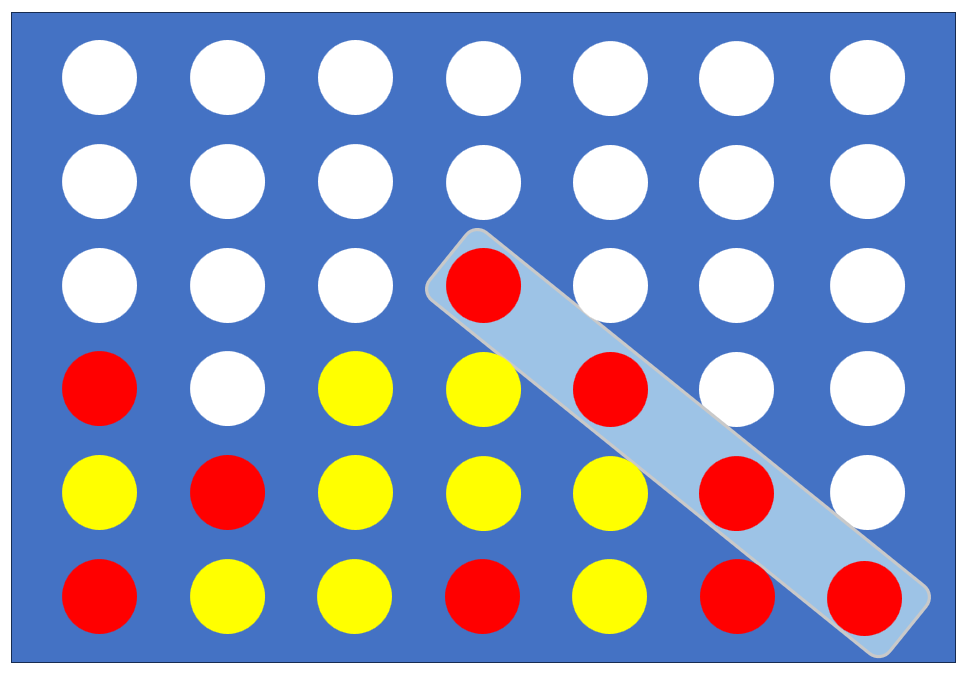
\includegraphics[width=\linewidth]{images/Diagonal}
	\caption[Vier rote Steine diagonal]{Vier rote Steine diagonal im Raster}
	\label{fig:diagonal}
\end{subfigure}\hfill
\begin{subfigure}{0.45\textwidth}
	\centering
	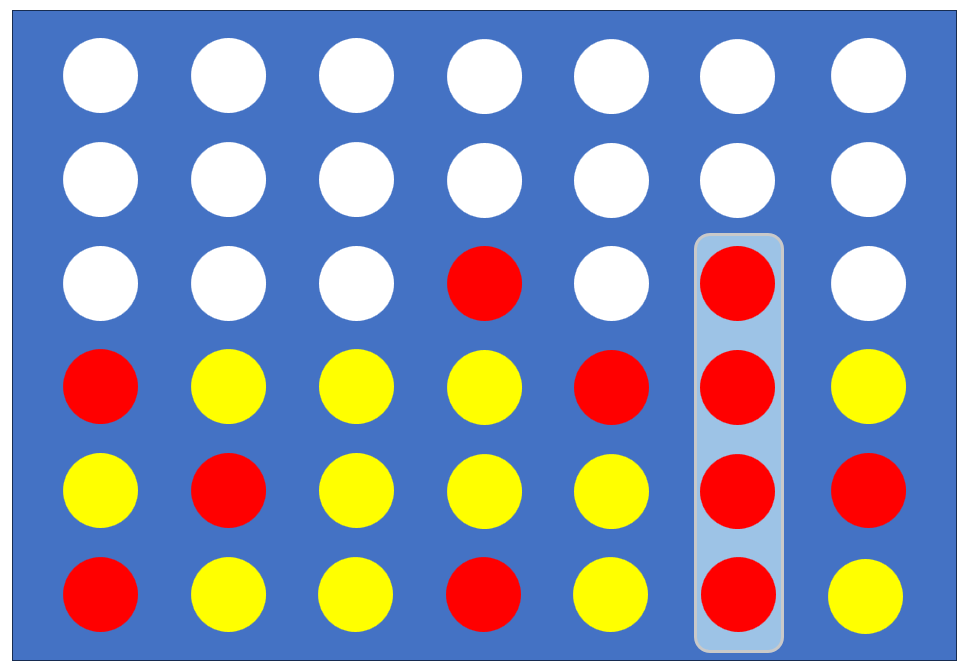
\includegraphics[width=\linewidth]{images/Senkrecht}
	\caption[Vier rote Steine in Reihe senkrecht]{Vier rote Steine senkrecht im Raster}
	\label{fig:senkrecht}
\end{subfigure}
\begin{subfigure}{0.45\textwidth}
	\centering
	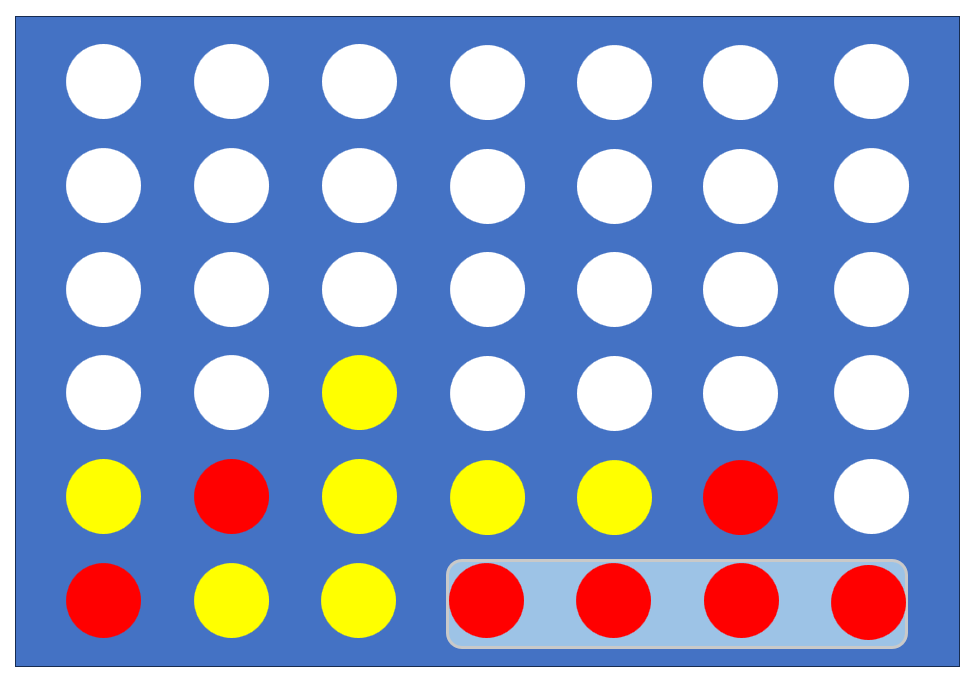
\includegraphics[width=\linewidth]{images/Waagrecht}
	\caption[Vier rote Steine in Reihe waagrecht]{Vier rote Steine waagrecht im Raster}
	\label{fig:waagrecht}
\end{subfigure}\hfill
\begin{subfigure}{0.45\textwidth}
	\centering
	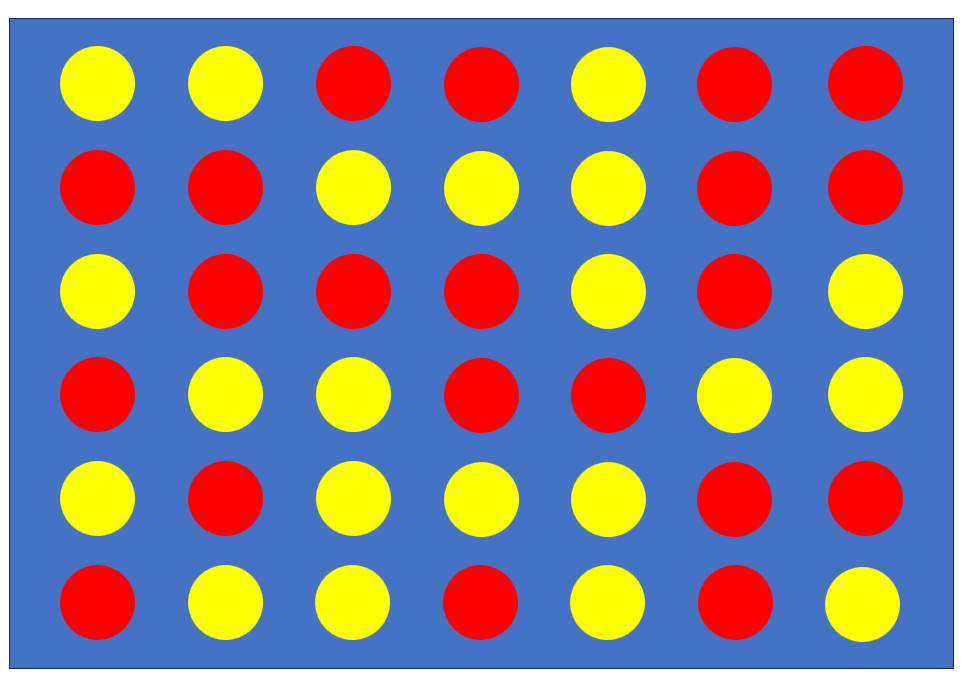
\includegraphics[width=\linewidth]{images/Unentschieden}
	\caption[Unentschieden]{Es kam keine vierer Reihe zustande}
	\label{fig:unentschiedent}
\end{subfigure}
\caption[Mögliche Spielausgänge]{Grafische Darstellung der möglichen Spielausgänge}
\end{figure}
%
%\newpage
\section{Historischer Hintergrund}
%Das Spiel “Vier Gewinnt” wurde 1973 von Howard Wexler und Ned Strongin entwickelt. Die Erstveröffentlichung erfolgte 1974 durch die Firma Milton Bradley, die im deutschsprachigen Raum als MB Spiele bekannt ist.
%Die Entwicklung des Spiels erfolgte durch die Strongin und Wexler Corporation in den USA. Obwohl der Preis der Erstausgabe nicht überliefert ist, wurde das Spiel schnell zu einem beliebten Strategiespiel.\\
%Eine interessante Entwicklung erfolgte bereits vor der Entstehung des klassischen Vier Gewinnt: 1967 erschien in den USA eine dreidimensionale Variante namens “Score Four”. Diese wurde 1974 in Deutschland von Ravensburger unter dem Namen “Sogo” vertrieben und war in der DDR als “Raummühle” bekannt.\\
%Das klassische Vier Gewinnt etablierte sich rasch als beliebtes Familienspiel und wurde über die Jahre in verschiedenen Varianten neu aufgelegt. Die Einfachheit der Regeln bei gleichzeitiger strategischer Tiefe trug maßgeblich zum anhaltenden Erfolg des Spiels bei.\\
%https://www.gameorama.ch/de/museum/spielmuseum/timeline/gewinnt?

Vier Gewinnt wurde 1973 von Howard Wexler und Ned Strongin entwickelt. Noch im selben Jahr lizenzierten die beiden Erfinder das Spiel an die Firma Milton Bradley, im deutschsprachigen Raum besser bekannt als ,,MB Spiele''
\autocite{gameorama_4gewinnt}\autocite{wikipedia_vier_gewinnt}.
Im darauffolgenden Jahr 1974 wurde das Spiel Vier Gewinnt von Milton Bradley veröffentlicht und in den Handel gebraucht. Das Spiel entwickelte sich seitdem zu einem der bekanntesten und beliebtesten Strategiespiele \autocite{wikipedia_vier_gewinnt}. Tatsächlich entwickelt es sich sogar zu einem echten Klassiker. Das Spiel ist beliebt bei Jung und Alt, da es recht leicht zu erlernen ist. Vier Gewinnt fördert die Konzentration und das logische Denken \autocite{50plus_vier_gewinnt}.
\newpage
Im Jahr 1967 erschien in den USA eine dreidimensionale Variante vom Spiel Vier Gewinnt, unter dem Namen ,,Score Four''. In Deutschland brauchte die Firma Ravensburger 1974 eine dreidimensionale Variante mit dem Namen ,,Sogo'' auf den Markt. (siehe Abbildung:\ref{fig:Sogo}) \
1988 wurde das Spiel von Victor Allis und James D. Allen nahezu gleichzeitig und unabhängig voneinander vollständig gelöst. Die Beiden haben mathematisch bewiesen, dass der erste Spieler bei fehlerfreiem Spiel immer gewinnen kann, wenn er den ersten Stein in der mittleren Spalte platziert.\autocite{wikipedia_vier_gewinnt}.
 
% \autocite{abebooks_image}
\begin{figure}[H]
	\centering
	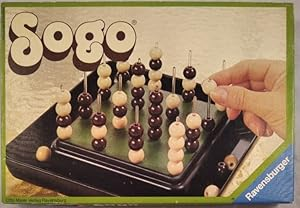
\includegraphics[width=0.8\linewidth]{images/Sogo}
	\caption[Sogo von Ravensburger \autocite{abebooks_image}]{dreidimensionale Variante ,,Sogo'' von Ravensburger}
	\label{fig:Sogo}
\end{figure}
\newpage

\section{Mathematische Eigenschaften des Spiels}
%Das Spiel 4Gewinnt weist mehrere wichtige mathematische Eigenschaften auf, die für seine Analyse fundamental sind.\\
%Hierbei liegt vorallem der Fokus auf Spielfeldgröße und Kombinatorik. Das klassische Spielfeld besteht aus 7 Spalten und 6 Reihen, was 42 mögliche Positionen ergibt. Diese Dimension wurde damals bewusst festgelegt, um ein ausgewogenes Verhältnis zwischen Komplexität und Spielbarkeit zu gewährleisten.\\
%
%Die Gesamtzahl der theoretisch möglichen Spielzustände lässt sich wie folgt berechnen:
%\begin{itemize}
%	\item Jede Position kann drei Zustände annehmen: leer, Spieler 1, Spieler 2
%	\item Dies ergibt theoretisch  mögliche Zustände\\
%	
%	Die tatsächliche Anzahl ist jedoch deutlich geringer, da:
%	\item Spielsteine nur von unten nach oben gesetzt werden können
%	\item Das Spiel endet, sobald vier Steine in einer Reihe liegen
%	\item Nicht alle Kombinationen sind durch legale Spielzüge erreichbar
%\end{itemize}
%
%Komplexitätsgrad
%•	Der durchschnittliche Verzweigungsfaktor (mögliche Züge pro Spielsituation) liegt bei etwa 4
%•	Die maximale Spieltiefe beträgt 42 Züge
%•	Die Spielbaumkomplexität ist deutlich geringer als bei Schach, aber höher als bei Tic-Tac-Toe
%Symmetrieeigenschaften
Das Spielfeld weist eine vertikale Symmetrie auf, wodurch sich die Anzahl der zu analysierenden Positionen reduziert. Die mittlere Spalte nimmt dabei eine besondere strategische Position ein.
%Diese mathematischen Eigenschaften bilden die Grundlage für die spieltheoretische Analyse und die Entwicklung von Lösungsstrategien.

Das Spiel 4Gewinnt weist mehrere mathematische Eigenschaften auf. Diese sind für eine Analyse des Spiels von Bedeutung. 
Das Strategiespiel ist ein Zwei-Personen-Nullsummenspiel. Das bedeutet, es spielen zwei Teilnehmer gegeneinander. Beide Spieler haben während des Spiels immer die volle Information über den Spielstand. Wenn einer von beiden gewinnt, bedeutet das gleichzeitig, dass der andere verloren hat.
Trotz der simplen Spielregeln ist vier Gewinnt dennoch recht komplex. Grund dafür die vielen möglichen Spielstellungen, es gibt nämlich ca. 4,5 Billionen mögliche Spielstellungen. Diese enorm hohe Anzahl an möglichen Spielstellungen kommt durch das Spielfeld mit sieben Spalten und sechs Reihen zustande.
Die Komplexität des Baumdiagramms liegt bei etwa $10^{21}$, was eine vollständige Analyse des Spielbaums sehr rechenintensiv macht \autocite{ruile2009viergewinnt}.

Das Lösen des Spiels Vier Gewinnt basiert auf verschiedenen mathematischen Techniken.
Zum einen gibt es die Anwendung des Zermelo-Bestimmtheitssatzes. Dieser besagt, dass entweder Spieler 1, Spieler 2 oder kein Spieler die Partie gewinnt. Im Kapitel \ref{sec:Analyse von Spielsituationen} wird näher auf den Bestimmtheitssatz eingegangen wird.\\
Eine weite Technik zur Analyse ist die Anwendung der Rückwärtsinduktion. Die Rückwärtsinduktion beginnt an der aktuellen Position und arbeitet sich zum Anfang zurück. Hierbei werden für jeden Spielzug die optimalen Entscheidungen der Spieler analysiert, unter der Berücksichtigung aller möglichen Züge.
Am Ende dieses Prozesses steht das beste Ergebnis für den beginnenden Spieler \autocite{mueller_2011}.\\
Die Rückwärtsinduktion wird durch die Payoff-Matrix-Analyse ergänzt. Das grundlegende Konzept der Payoff-Matrix-Analyse bietet eine Möglichkeit zur Darstellung strategischer Interaktionen und Entscheidungen dar \autocite{fasterCapital2024}.


\begin{center}
	\begin{figure}[h]
		\centering
		\begin{tabular}{cc|c|c|c}
			\multicolumn{1}{c}{} & \multicolumn{4}{c}{\textcolor{blue}{Spieler 2}} \\
			&	& Zentrum & Rand & Defensiv \\
			\cline{2-5}
			\multirow{3}{*}{\rotatebox{90}{\textcolor{red}{Spieler 1}}} & Zentrum & $(\textcolor{red}{0},\textcolor{blue}{0})$ & $(\textcolor{red}{1},\textcolor{blue}{-1})$ & $(\textcolor{red}{0},\textcolor{blue}{0})$ \\
			\cline{3-5}
			&Rand& $(\textcolor{red}{-1},\textcolor{blue}{1})$ & $(\textcolor{red}{0},\textcolor{blue}{0})$ & $(\textcolor{red}{-1},\textcolor{blue}{1})$ \\
			\cline{3-5}
		&Defensiv& $(\textcolor{red}{0},\textcolor{blue}{0})$ & $(\textcolor{red}{1},\textcolor{blue}{-1})$ & $(\textcolor{red}{0},\textcolor{blue}{0})$ \\
		\end{tabular}\\
		\caption[Payoff-Matrix für Vier gewinnt]{Payoff-Matrix für Vier gewinntt}
		\label{fig:payoff}
	\end{figure}
\end{center}

\begin{minipage}{\linewidth}
	\centering
	 \textbf{Legende der Payoff-Matrix}\\
	\textcolor{red}{Rot} = Spieler 1, \textcolor{blue}{Blau} = Spieler 2,\\
	1=Vorteil, 0=Neutral, -1=Verlust
\end{minipage}
 